\section{Das Minimalgerüst-Problem / Minimum Spanning Tree Problem}

Gegeben sei ein ungerichteter, zusammenhängender und gewichteter Graph $G = (V,E,c)$, wobei $\abb{c}{E}{\R}$ die Gewichtsfunktion ist.

Gesucht ist eine Teilmenge $T \subseteq E$ mit $\card{T} = \card{V} - 1$, sodass der induzierte Teilgraph $G_T = (V,T)$ kreisfrei ist.

\begin{definition}
	Jede Teilmenge $T$ mit diesen Eigenschaften wird \begriff{Gerüst} oder \begriff{Spannbaum} genannt.
\end{definition}

\begin{bemerkung}
	Der zu einem Spannbaum $T$ gehörende Teilgraph $G_T$ ist zusammenhängend.
\end{bemerkung}

Das Minimum-Spanning-Tree (MST) Problem besteht nun darin, einen Spannbaum zu finden, dessen Gesamtgewicht $\sum_{e \in T} c(e)$ kleinstmöglich ist. Es lässt sich mithilfe eines sogenannten \begriff{Greedy-Algorithmus} effizient lösen. Diese Algorithmen zeichnen sich vor allen dadurch aus, dass sie schrittweise denjenigen Folgezustand wählen, der \enquote{lokal} (also zum Zeitpunkt der Auswahl) das beste Ergebnis verspricht. Derartige Algorithmen sind oft sehr schnell, lösen das Problem aber im Allgemeinen nicht optimal. Im Falle des MST-Problems führt jedoch das folgende Verfahren stets zur optimalen Lösung.

\subsection{Algotihmus von \person{Kruskal}}

\textbf{Idee:} Wähle in jeder Iteration eine Kante mit kleinstem Gewicht, wobei kein Kreis entstehen darf. Formal verfahren wir also wie folgt.

\fbox{\textbf{Algorithmus von \person{Kruskal}:}}
\begin{enumerate}[label=Schritt \arabic*:, leftmargin=*, start=0]
	\item Initialisierung: $T \defeq \emptyset$
	\item Solange $\card{T} < n -1$: ermittle eine Kante $e \in E$ mit kleinstem Gewicht $c(e)$, setze $E \defeq E \setminus \menge{e}$ und, falls $T \cup \menge{e}$ kreisfrei ist, setze $T \defeq T \cup \menge{e}$.
\end{enumerate}

Der Aufwand dieses Algorithmus wird maßgeblich von der Sortierung der Kantengewichte beeinflusst und lässt sich mit $\mathcal{O}(\card{E} * \log\card{E})$ abschätzen. Die Überprüfung der Kreisfreiheit ist bei geschickter Implementierung \enquote{schneller} durchführbar.

\begin{beispiel}
	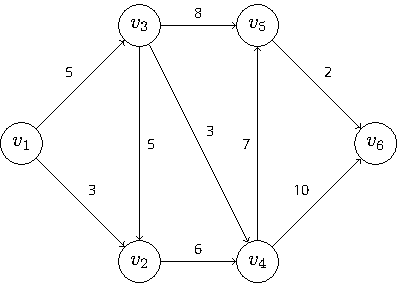
\includegraphics[width=.3\textwidth]{optinum_abb/optinum_5_2_bsp5-1.pdf}
	
	Jeder minimale Spannbaum hat ein Gewicht von $c = 2+3+3+4+7 = 20$.
\end{beispiel}

\subsection{Algorithmus von \person{Prim} \& \person{Dijkstra}}

Eine alternative Vorgehensweise zur Gewinnung eines minimalen Spannbaums, bei der in jedem Schritt auf den Zusammenhang des Graphen $G_T$ geachtet wird, kann wie folgt beschrieben werden.

\fbox{\textbf{Algorithmus von Prim \& Dijkstra}}
\begin{enumerate}[label=Schritt \arabic*:, leftmargin=*, start=0]
	\item Initialisierung: $T \defeq \emptyset$, $S \defeq \menge{u}$ für ein beliebiges $u \in V$. Für alle $v \in V \setminus \menge{u}$ setze
	\begin{itemize}[nolistsep, topsep=-\parskip]
		\item $h(v) \defeq c(u,v)$, $p(v) \defeq u$ \hspace{1em} falls $\menge{u,v} \in E$
		\item $h(v) \defeq + \infty$ \hspace{1em} sonst
	\end{itemize}
	\item Solange $\card{T} < n -1$: bestimme $v \in V \setminus S$ mit $h(v) = \min\menge{h(t) : t \in V \setminus S}$ und setze $T \defeq T \cup \menge{\menge{p(v),v}}$ sowie $S \defeq S \cup \menge{v}$. Für alle $t \in V \setminus S$ mit $\menge{v,t} \in E$ und $c(v,t) < h(t)$ setze $h(t) \defeq c(v,t)$, $p(t) \defeq v$.
\end{enumerate}

Dieser Algorithmus ist ebenfalls ein Greedy-Verfahren und besitzt (bei \enquote{gewöhnlicher} Implementierung) eine Laufzeit von $\mathcal{O}(\card{V}^2)$, jedoch sind bei Verwendung spezieller Datenstrukturen auch bessere Abschätzungen möglich. Beide Algorithmen beginnen mit einer leeren Knotenmenge und fügen in jedem Schritt eine Kante mit minimalem \enquote{Gewicht} ($c$ bzw. $h$) hinzu. Sie unterscheiden sich vor allem darin, wie genau die Auswahl dieser Kante erfolgt und wie die Bildung eines Kreises vermieden wird.
